\problemname{\problemyamlname}

The great city of Karwa-upon-Thyne would like to modernize the buildings along the dyke.
Indeed, the city would like to place solar panels on these buildings and, so as to take advantage of the electrical production of these as much as possible, it decides to cover the roofs as well as the \textbf{side} facades.

To this end, you've been hired in order to determine how many meters of solar panel the city will need.
The city gives you a side-view of the dyke, specifying the size of each building like this :

For each 1 meter wide spot, the plan gives you the height of the building at that spot as shown in the figure below.

\begin{figure}[h]
\centering
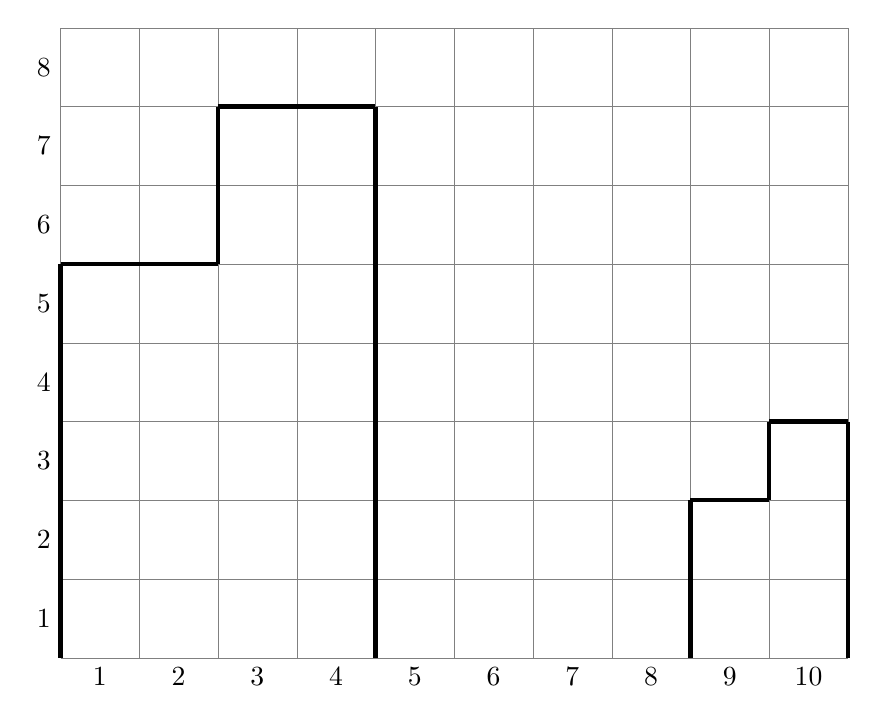
\begin{tikzpicture}
\draw[step=1.0, gray, ultra thin] (0,0) grid (10, 8);

  \draw[ultra thick] (0,0) -- (0, 5);
  \draw[ultra thick] (0, 5) -- (2, 5);
  \draw[ultra thick](2,5) -- (2, 7);
  \draw[ultra thick](2, 7) -- (4, 7);
  \draw[ultra thick](4,7) -- (4, 0);
  \draw[ultra thick](8,0) -- (8, 2);
  \draw[ultra thick](8, 2) -- (9, 2);
  \draw[ultra thick](9, 2) -- (9, 3);
  \draw[ultra thick] (9, 3) -- (10, 3);
  \draw[ultra thick] (10, 3) -- (10, 0);

    \foreach \x in {1, ..., 10} {%
      % Bottom
      \node[anchor=north] at (\x-0.5,0) {\x};
    }
    
    \foreach \y in {1, ..., 8} {%
      % Left
      \node[anchor=east] at (0,\y-0.5) {\y};
    }
\end{tikzpicture}
\newline
\textit{Illustration of the first example \\ In black is where the city would like to lay solar panels.}
\end{figure}

\begin{Input}
	The input consists of;
	\begin{itemize}
		\item One line with an integer $n$ ($1 \le n \le 10^4$), the length of the dyke.
		\item A second line which represents the horizon line, composed of $n$ integers $h_i$ ($0 \le h_i \le 100$) separated by a space representing the height of the building $i$.
	\end{itemize}
\end{Input}

\begin{Output}
	The integer representing the number of meters of solar panel necessary in order to cover the totality of the sides and the tops of the buildings.
\end{Output}

%%% Local Variables:
%%% mode: latex
%%% TeX-master: t
%%% End:
